\documentclass[11pt,a5paper,landscape]{article}

\usepackage{main}
\usepackage{exercices}

\renewcommand{\typedocument}{Exercices}
\renewcommand{\classe}{3e}
\renewcommand{\titre}{Exercices - Mouvement et vitesse}

\begin{document}
\begin{multicols*}{2}

% ----- Exercice 1 -----

\exercice{Vecteur vitesse}
Dans chaque cas, préciser si la direction et/ou la valeur du mouvement varie au cours du temps.
\begin{enumerate}
    \item Un athlète fait des tours de piste. Le mouvement est uniforme.
    \item Une voiture freine sur une route droite.
\end{enumerate}

% ----- Exercice 2 -----

\exercice{Calcul de vitesse}
\begin{enumerate}
    \item Convertir 1 km/h en m/s puis 1 m/s en km/h.
\end{enumerate}
Dans chaque cas, calculer la vitesse en m/s et en km/h:
\begin{enumerate}
    \setcounter{enumi}{1}
    \item Une voiture parcourt un tronçon d’autoroute de 240km en 2h.
    \item Un piéton marche 14km en 3h30.
    \item Un escargot prend 40 minutes pour faire 6m.
\end{enumerate}

% ----- Exercice 3 -----

\exercice{Vitesse de la lumière}
Données :
\begin{itemize}
    \item Vitesse de la lumière dans le vide : $3,00\times10^8 m/s$
    \item Distance Terre-Soleil : $150\times10^9m$
\end{itemize}

\begin{enumerate}
    \item Calculer le temps que met la lumière du Soleil pour atteindre la Terre.
    \item Combien de temps mettraient la voiture, le piéton et l'escargot de l'exercice 2 ?
\end{enumerate}
Une année-lumière correspond à la distance parcourue par la lumière en une année.
\begin{enumerate}
    \setcounter{enumi}{2}
    \item Quelle est la grandeur d'une année-lumière ?
    \item Peut-on dire : "Il est lent, on l'attend depuis 3 années-lumières." ? Pourquoi ?
    \item Convertir une année-lumière en km.
\end{enumerate}

% ----- Exercice 4 -----

\exercice{Vitesse moyenne}
Un randonneur fait l’ascension et la descente d’une montagne. Il marche à 4km/h à l’aller et à 6km/h au retour en empruntant le même chemin. Quelle est sa vitesse moyenne ? Le démontrer par le calcul.

% ----- Exercice 5 -----

\exercice{Référentiel}
Les escalators parcourent 15m en 10s. \\

\begin{minipage}{5cm}
    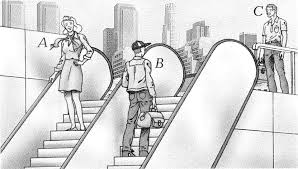
\includegraphics[width=5cm]{images/escalators mouvement.jpg}
\end{minipage}
\hfill
\begin{minipage}{5cm}
    \begin{enumerate}
        \item Par rapport au référentiel terrestre, qui est en mouvement ?
        \item Quelle est la vitesse de A par rapport à C ? Par rapport à B ?
    \end{enumerate}
\end{minipage}

\end{multicols*}
\end{document}